\documentclass[t]{beamer}
\usepackage[utf8]{inputenc}  % to be able to type unicode text directly
%\usepackage[french]{babel}   % french typographical conventions
\usepackage{inconsolata}     % for a nicer (e.g. non-courier) tt family font
%\usepackage{amsthm,amsmath}  % fancier mathematics
\usepackage{array} % to fine-tune tabular spacing
\usepackage{bbm} % for blackboard 1

\usepackage{graphicx}        % to include images
%\usepackage{animate}         % to include animated images
\usepackage{soul}            % for colored strikethrough
%\usepackage{bbding}          % for Checkmark and XSolidBrush
\usepackage{hyperref,url}

\colorlet{darkgreen}{black!50!green}  % used for page numbers
\definecolor{term}{rgb}{.9,.9,.9}     % used for code insets

\setlength{\parindent}{0em}
\setlength{\parskip}{1em}


% coco's macros
\def\R{\mathbf{R}}
\def\F{\mathcal{F}}
\def\x{\mathbf{x}}
\def\y{\mathbf{y}}
\def\u{\mathbf{u}}
\def\Z{\mathbf{Z}}
\def\d{\mathrm{d}}
\DeclareMathOperator*{\argmin}{arg\,min}
\DeclareMathOperator*{\argmax}{arg\,max}
\newcommand{\reference}[1] {{\scriptsize \color{gray}  #1 }}
\newcommand{\referencep}[1] {{\tiny \color{gray}  #1 }}
\newcommand{\unit}[1] {{\tiny \color{gray}  #1 }}

% disable spacing around verbatim
\usepackage{etoolbox}
\makeatletter\preto{\@verbatim}{\topsep=0pt \partopsep=0pt }\makeatother

% disable headings, set slide numbers in green
\mode<all>\setbeamertemplate{navigation symbols}{}
%\defbeamertemplate*{footline}{pagecount}{\leavevmode\hfill\color{darkgreen}
%   \insertframenumber{} / \inserttotalframenumber\hspace*{2ex}\vskip0pt}

%% select red color for strikethrough
\makeatletter
\newcommand\SoulColor{%
  \let\set@color\beamerorig@set@color
  \let\reset@color\beamerorig@reset@color}
\makeatother
\newcommand<>{\St}[1]{\only#2{\SoulColor\st{#1}}}
\setstcolor{red}

% make everything monospace
\renewcommand*\familydefault{\ttdefault}

\begin{document}

\begin{frame}
IMPLICIT IMAGE MODELS OF CLASSICAL DENOISERS\hfill{\footnotesize{\color{gray}mnhrdt}}\\
============================================

\small
Any denoiser contains an ``implicit image prior''.\\
How can we can extract images from it?

{\color{gray}Kadkhodaie--Simoncelli 2021}\\
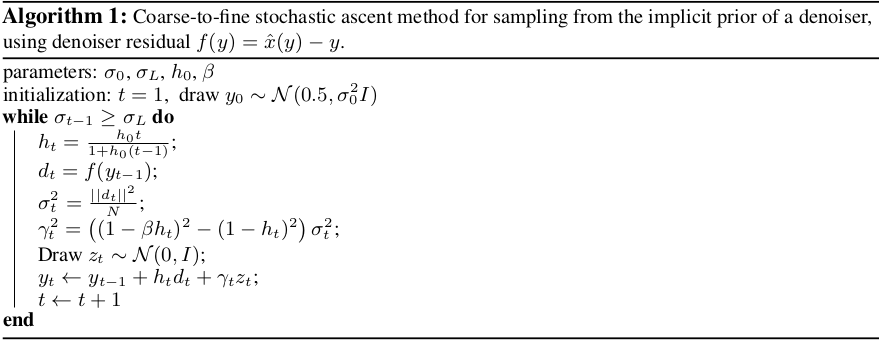
\includegraphics[width=0.7\linewidth]{ks.png}

%\vfill
{\bf Demo: } Bring your own denoiser for this algorithm

%\vfill
\tiny
\begin{tabular}{lll}
	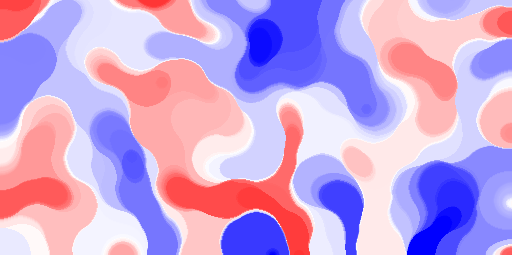
\includegraphics[height=0.18\textheight]{somiters3b.png} &
	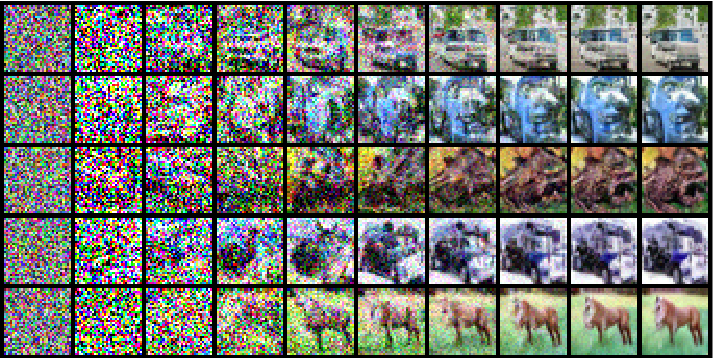
\includegraphics[height=0.18\textheight]{songermon1b.png} &
	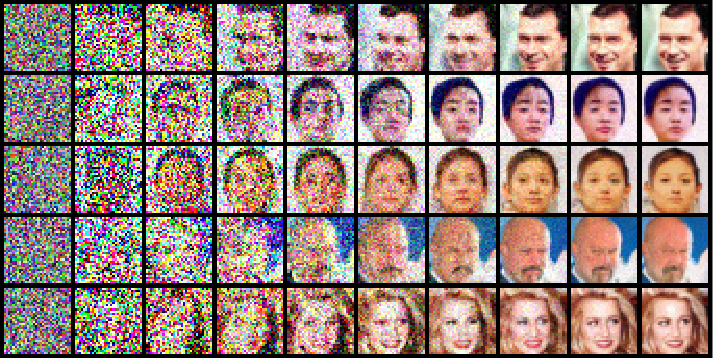
\includegraphics[height=0.18\textheight]{songermon1a.png} \\
	Denoiser = median &
	Denoiser = DCNN (generic) &
	Denoiser = DCNN (faces)
\end{tabular}

\end{frame}


\end{document}


% vim:sw=2 ts=2 spell spelllang=fr:
